
%!TeX spellcheck = en-US
%!TEX root = ../hw1_report.tex

It is evident from Figure \ref{fig:task7a1k5}--\ref{fig:task7a2k10} that convergence of the approximation of eigenvalues can't be expected. We see that round-off errors heavily affects the convergence, however this is expected for explicit restart.

The idea of restart is to be able to use a smaller $m$ by restarting the Arnoldi method with a new starting vector based on the Ritz vectors from the previous run. In the explicit case the the vector is a linear combination of the Ritz vectors corresponding to the $k$ largest Ritz values in modulus.

In the implicit case the Arnoldi method is not entirely restarted. Instead it only keeps the first $p$ to continue, i.e.

\begin{equation*}
  A Q_{m} = Q_{m+1} \underline{H}_{m} \rightarrow A Q_{p} = Q_{p+1} \underline{H}_{p}
\end{equation*}
where $Q_{p}$ and $Q_{p+1}$ are transformations of $Q_{m}$ and $Q_{m+1}$, respectively.
From \ref{fig:task7b1k5}--\ref{fig:task7b2k10} we see that the approximation of the eigenvalues indeed converges after $8$ and $10$ iterations. For the latter we used $m = 16$, instead of $20$, as the method breaks down for $20$. For $p = 18$ one of the approximate eigenvalues started to deviate at the $18$:th iteration, which could be due to immediate break down.

We see that implicit restart indeed circumvents the instabilities that polute the explicit restart method, and should thus be used instead.

\begin{figure}[h!]
\centering
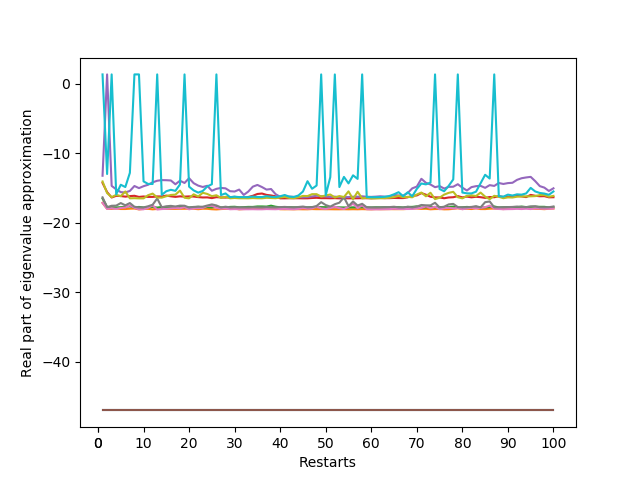
\includegraphics[scale=0.4]{../task7/task7a1_k5m10.png}
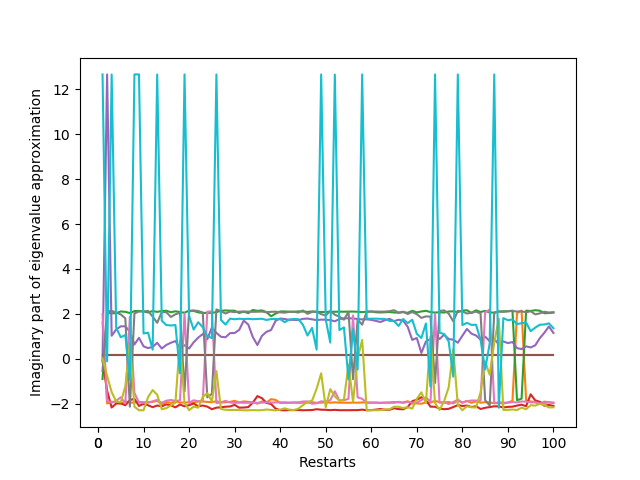
\includegraphics[scale=0.4]{../task7/task7a2_k5m10.png}
\caption{The evolution of eigenvalue approximation for $\lambda_{i}$, $i = 1,\ldots,m$ with explicit restart for $k = 5$ and $m=10$.}
\label{fig:task7a1k5}
\end{figure}


\begin{figure}[h!]
\centering
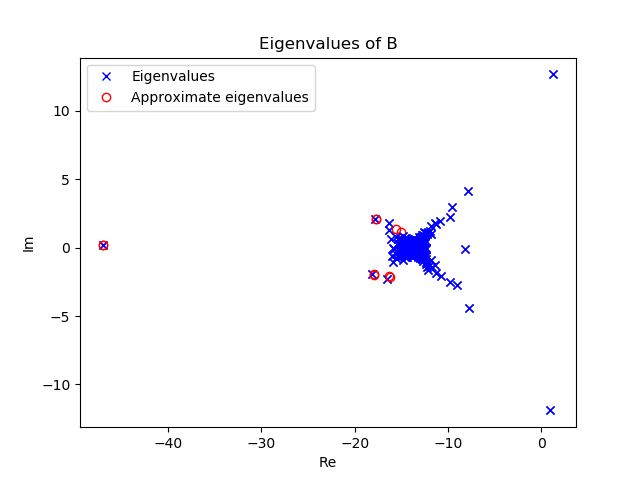
\includegraphics[scale=0.8]{../task7/task7a3_k5m10.png}
\caption{Explicit restart: Plot of eigenvalue approximation for $\lambda_{i}$, $i = 1,\ldots,m$ for $k = 5$ and $m=10$.}
\label{fig:task7a2k5}
\end{figure}



\begin{figure}[h!]
\centering
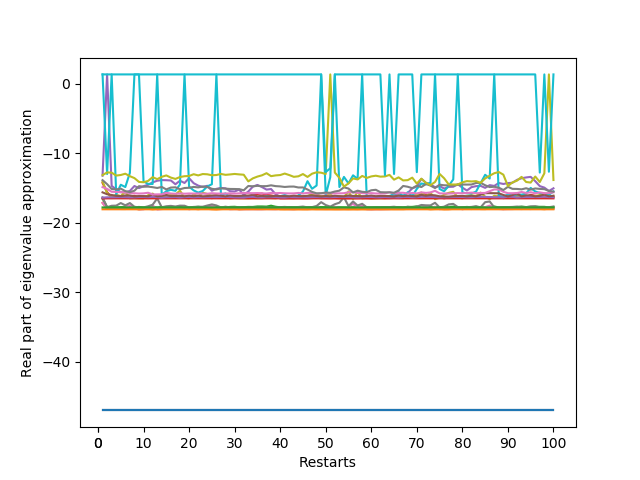
\includegraphics[scale=0.4]{../task7/task7a1_k10m20.png}
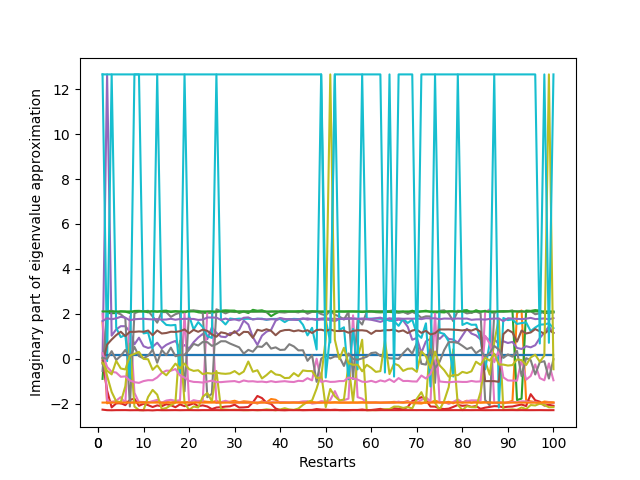
\includegraphics[scale=0.4]{../task7/task7a2_k10m20.png}
\caption{The evolution of eigenvalue approximation for $\lambda_{i}$, $i = 1,\ldots,m$ with explicit restart for $k = 10$ and $m=20$.}
\label{fig:task7a1k10}
\end{figure}


\begin{figure}[h!]
\centering
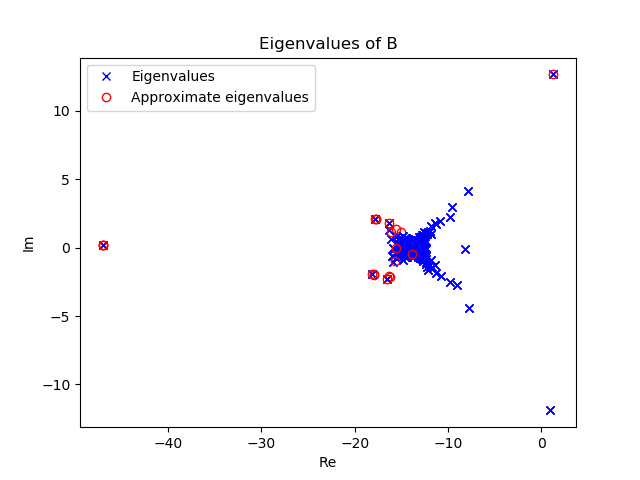
\includegraphics[scale=0.8]{../task7/task7a3_k10m20.png}
\caption{Explicit restart: Plot of eigenvalue approximation for $\lambda_{i}$, $i = 1,\ldots,m$ for $k = 10$ and $m=20$}.
\label{fig:task7a2k10}
\end{figure}

%IMPLICIT

\begin{figure}[h!]
\centering
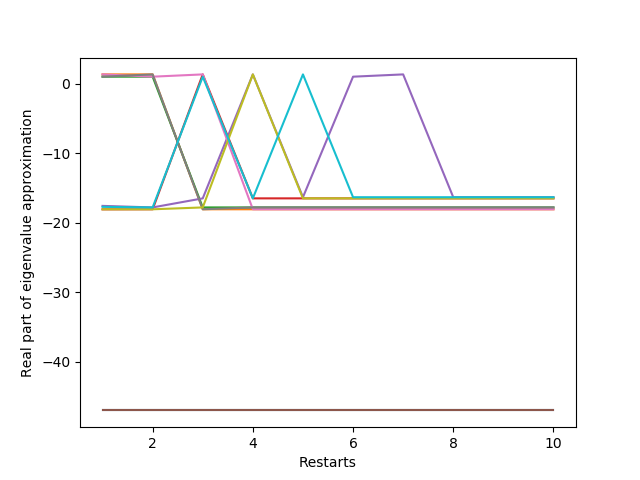
\includegraphics[scale=0.4]{../task7/task7b1_k5m10p10.png}
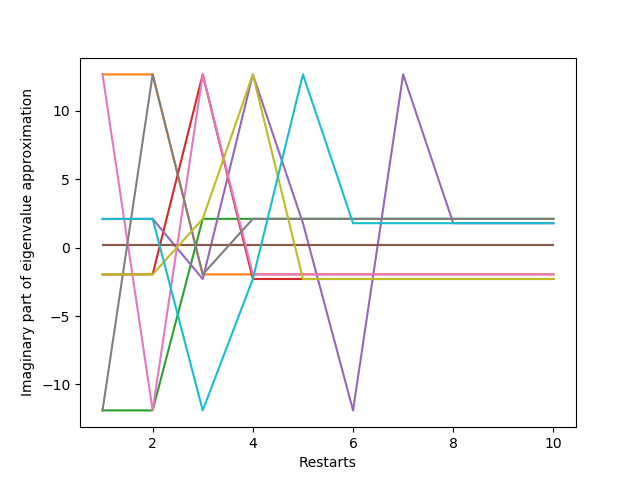
\includegraphics[scale=0.4]{../task7/task7b2_k5m10p10.png}
\caption{The evolution of eigenvalue approximation for $\lambda_{i}$, $i = 1,\ldots,m$ with implicit restart for $k = 5$, $m=10$ and $p = 10$.}
\label{fig:task7b1k5}
\end{figure}


\begin{figure}[h!]
\centering
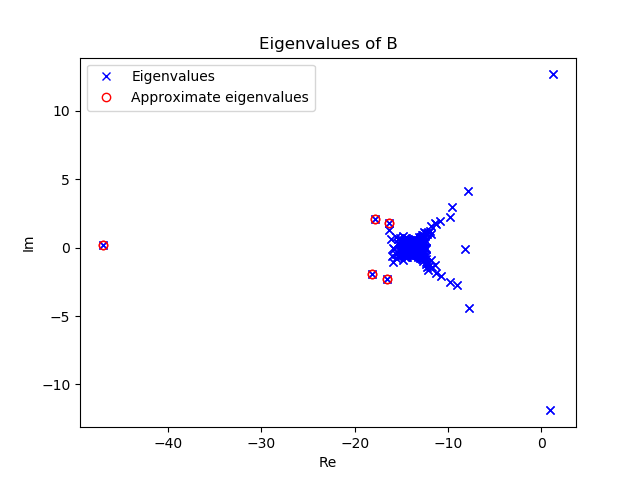
\includegraphics[scale=0.8]{../task7/task7b3_k5m10p10.png}
\caption{Implicit restart: Plot of eigenvalue approximation for $\lambda_{i}$, $i = 1,\ldots,m$ for $k = 5$, $m=10$ and $p = 10$.}
\label{fig:task7b2k5}
\end{figure}



\begin{figure}[h!]
\centering
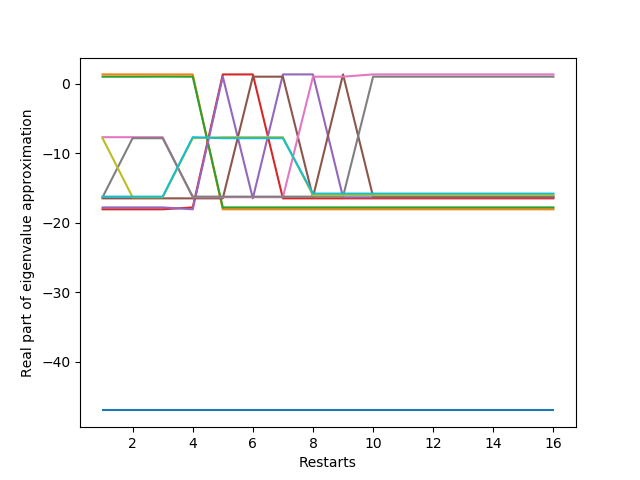
\includegraphics[scale=0.4]{../task7/task7b1_k10m16p20.png}
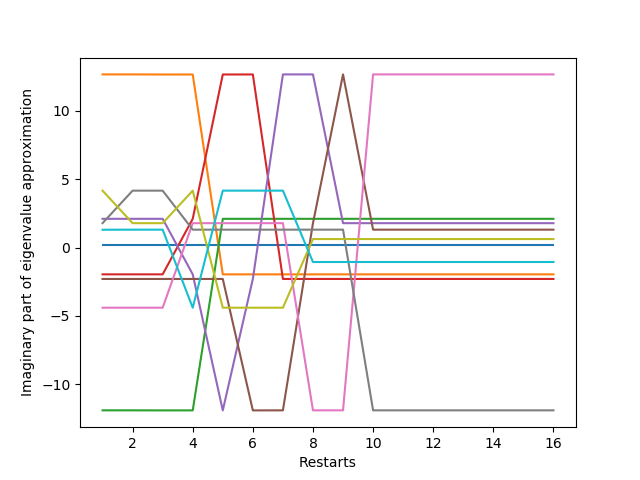
\includegraphics[scale=0.4]{../task7/task7b2_k10m16p20.png}
\caption{The evolution of eigenvalue approximation for $\lambda_{i}$, $i = 1,\ldots,m$ with implicit restart for $k = 10$, $m=16$ and $p = 20$.}
\label{fig:task7b1k10}
\end{figure}


\begin{figure}[h!]
\centering
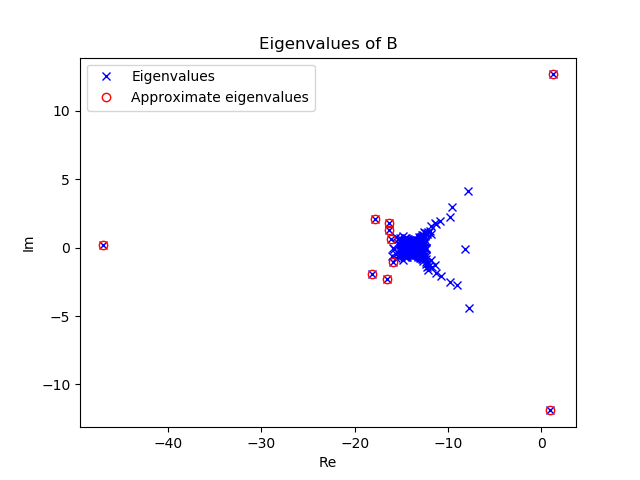
\includegraphics[scale=0.8]{../task7/task7b3_k10m16p20.png}
\caption{Implicit restart: Plot of eigenvalue approximation for $\lambda_{i}$, $i = 1,\ldots,m$ for $k = 10$, $m=16$ and $p = 20$.}
\label{fig:task7b2k10}
\end{figure}






% \begin{figure}[h!]
% \centering
% 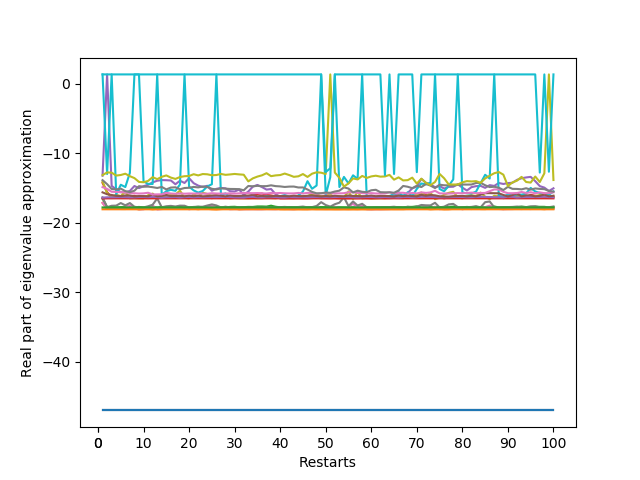
\includegraphics[scale=0.4]{../task7/task7a1_k10m20.png}
% 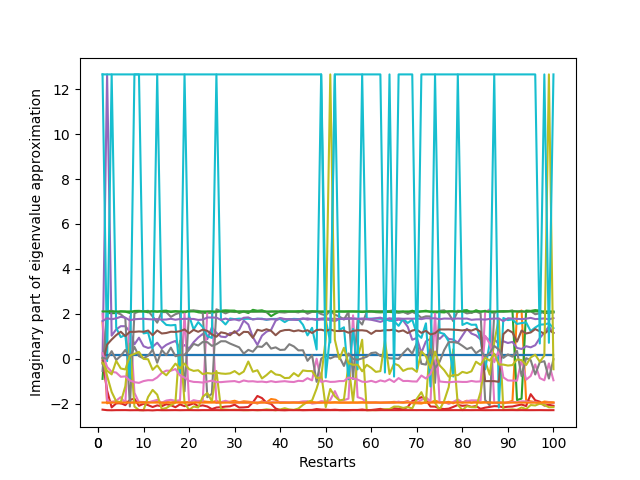
\includegraphics[scale=0.4]{../task7/task7a2_k10m20.png}
% \caption{The convergence of eigenvalue approximation for $\lambda_{i}$, $i = 1,\ldots,5$ for $k = 5$ and $m=10$}
% \label{fig:task7a1}
% \end{figure}
%
%
% \begin{figure}[h!]
% \centering
% 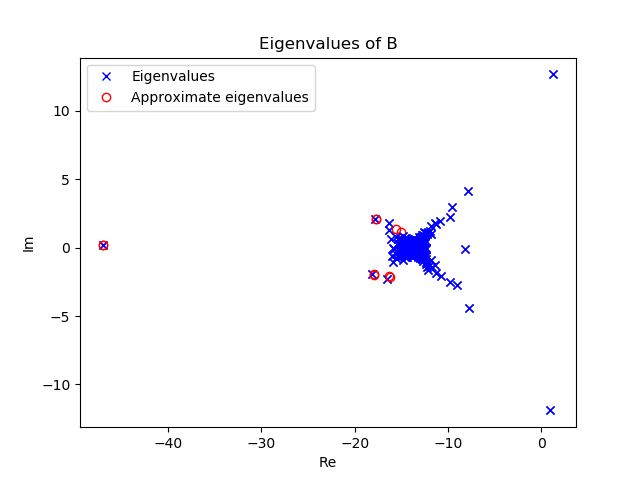
\includegraphics[scale=0.8]{../task7/task7a3_k5m10.png}
% \caption{Plot of eigenvalue approximation for $\lambda_{i}$, $i = 1,\ldots,5$ for $k = 5$ and $m=10$}
% \label{fig:task7a2}
% \end{figure}
